\documentclass[tikz,border=2pt]{standalone}
\usetikzlibrary{shapes.geometric, arrows, graphs, graphs.standard, positioning, decorations.markings, calc}

\tikzset{
    box/.style = {draw, rectangle, rounded corners, minimum width=1.1cm, minimum height=4cm, outer sep=2mm},
    cir/.style = {draw, circle, minimum size=.75cm, align=center, outer sep=2mm, inner sep=0.2em},
    arr/.style = {-},
    shorten/.style = {shorten <=#1, shorten >=#1},
    dots/.style= {decoration={markings, mark= between positions 0 and 1 step 2mm with {\fill circle (0.75mm);}},decorate}
}

\begin{document}
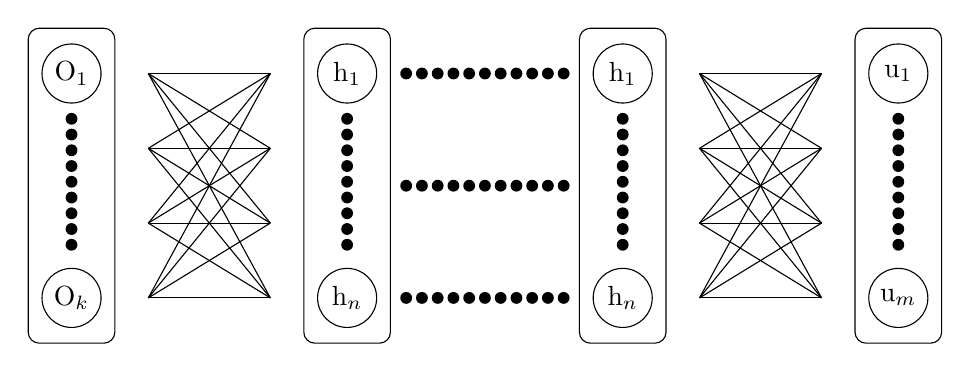
\begin{tikzpicture}
    \def\circlesep{2mm}
    \def\boxsep{2cm}
    \node (box11) [box] {};
    \node (cir11) [cir,below=\circlesep] at (box11.north) {O$_1$};
    \node (cir12) [cir,above=\circlesep] at (box11.south) {O$_k$};
    \draw[dots] (cir11) -- (cir12);

    \node (box21) [box,right=\boxsep of box11] {};
    \node (cir21) [cir,below=\circlesep] at (box21.north) {h$_1$};
    \node (cir22) [cir,above=\circlesep] at (box21.south) {h$_n$};
    \draw[dots] (cir21) -- (cir22);

    \node (box31) [box,right=\boxsep of box21] {};
    \node (cir31) [cir,below=\circlesep] at (box31.north) {h$_1$};
    \node (cir32) [cir,above=\circlesep] at (box31.south) {h$_n$};
    \draw[dots] (cir31) -- (cir32);

    \node (box41) [box,right=\boxsep of box31] {};
    \node (cir41) [cir,below=\circlesep] at (box41.north)  {u$_1$};
    \node (cir42) [cir,above=\circlesep] at (box41.south) {u$_m$};
    \draw[dots] (cir41) -- (cir42);

    \draw[dots] (cir21.east -| box21.east) -- (cir31.west -| box31.west);
    \draw[dots] (box21.east) -- (box31.west);
    \draw[dots] (cir22.east -| box21.east) -- (cir32.west -| box31.west);

    \path[shift={([xshift=.4cm]cir11.east)}] let \p1=($([xshift=.4cm]cir11.east)$),\p2=($([xshift=-.4cm]cir22.west)$),
                                                 \n1={\x2-\x1}, \n2={(\y1-\y2)/3} in graph[nodes={coordinate},
                                                                                           empty nodes,
                                                                                           grow right=\n1,
                                                                                           branch down=\n2]{subgraph K_nm [n=4, m=4]};
    \path[shift={([xshift=.4cm]cir31.east)}] let \p1=($([xshift=.4cm]cir31.east)$), \p2=($([xshift=-.4cm]cir42.west)$),
                                                 \n1={\x2-\x1}, \n2={(\y1-\y2)/3} in graph[nodes={coordinate},
                                                                                           empty nodes,
                                                                                           grow right=\n1,
                                                                                           branch down=\n2]{subgraph K_nm [n=4, m=4]};
\end{tikzpicture}
\end{document}
